\documentclass[12pt]{article}
%%% DOCUMENT FORMATTING %%%
\usepackage[margin=1in]{geometry}
\usepackage{enumitem}
\setlength{\parindent}{0pt}
\newcommand{\disp}{\displaystyle}

%%% HEADER %%%
\usepackage{fancyhdr}
\pagestyle{fancy}
\fancyhf{}
\lhead{MATH 1060}
\rhead{Vagnozzi}
\cfoot{\thepage}

%%% MATH NOTATION & SYMBOLS %%%
\usepackage{amssymb}
\usepackage{amsmath}
\newcommand{\R}{\mathbb{R}}
\newcommand{\N}{\mathbb{N}}
\newcommand{\Z}{\mathbb{Z}}
\newcommand{\lp}{\left(}
\newcommand{\rp}{\right)}
\newcommand{\ls}{\left[}
\newcommand{\rs}{\right]}
\newcommand{\lb}{\left\{}
\newcommand{\rb}{\right\}}
\newcommand{\arccot}{\text{arccot}}
\newcommand{\arccsc}{\text{arccsc}}
\newcommand{\arcsec}{\text{arcsec}} 

%%% TABLES %%%
\usepackage{colortbl}

%%% GRAPHS %%%
\usepackage{tikz}
\usepackage{pgfplots}
\pgfplotsset{compat=1.15}
\usepgfplotslibrary{fillbetween}
\usetikzlibrary{angles,quotes}

%%% ENVIRONMENTS %%%
\newcommand{\Example}{\paragraph{\Writinghand \hspace{0.1mm} Example.}}
\newcommand{\ExampleCont}{\paragraph{\Writinghand \hspace{0.1mm} Example (continued).}}
\newcommand{\boxenv}[2]{
	\fbox{
	\begin{minipage}{0.97\textwidth}
	\vspace{2mm}	
	\paragraph{#1} #2
	\vspace{2mm}
	\end{minipage}
	}}

%%% FUN THINGS %%%
\newcommand*\tc[1]{\tikz[baseline=(char.base)]{
            \node[shape=circle,draw,inner sep=2pt] (char) {#1};}}
\usepackage{marvosym}

%%% MISC %%%
\usepackage{hyperref}


\setcounter{page}{16}

\begin{document}
\section*{2.1: The Idea of Limits}

\boxenv{Learning Objectives.}{Upon successful completion of Section 2.1, you will be able to\dots
		
	\begin{itemize}[leftmargin=6mm]
		\item Answer conceptual questions involving average velocity or secant and tangent lines.
		\item Calculate average and instantaneous velocities.
		\item Calculate slopes of secant and tangent lines.
		\item Solve applications involving average and instantaneous velocities.
	\end{itemize}
	\vspace{-4mm}
}

\vspace{5mm}

\subsection*{The Idea of a Limit}
Given a function $f$ and some input $x=c$ in the domain of $f$, we are able to calculate the $y$-value, i.e.\ $f(c)$. For instance, if $f(x)=3x-1$, then\dots

\vspace{15mm}

However, in some cases, things might not work out as nicely. Consider instead the function $f(x)=\disp\frac{x^2-9}{x-3}$. Because $x=3$ is not in the domain of $f$, we cannot calculate $f(3)$.

\vspace{15mm}

Very informally, we might say that the ``limit'' of $f(x)$ at $x=3$ is what $f(3)$ ``should'' be. As you learn about how to work with limits, you will be able to show the following.

$$\lim_{x\to 3}\frac{x^2-9}{x-3}=6$$

\vspace{5mm}

\subsection*{Exploring Limits}
We will explore the idea of a limit through the concept of velocity. The \textbf{average velocity} on some time interval $\ls t_1,t_2\rs$ is as follows.
$$v_{\text{avg}}=\frac{\text{distance traveled}}{\text{time elapsed}}=\frac{\Delta s}{\Delta t}=\frac{s(t_2)-s(t_1)}{t_2-t_1}$$

\Example The position of a rock $t$ seconds after being launched at a speed of 96 ft/s is given by $s(t)=-16t^2+96t$ feet. The average velocity between $t=1$ and $t=3$ is\dots

\newpage 

\textbf{Geometric Interpretation.} Geometrically, this average velocity is the slope of the line passing through the points $(1,80)$ and $(3,144)$.

\begin{center}
            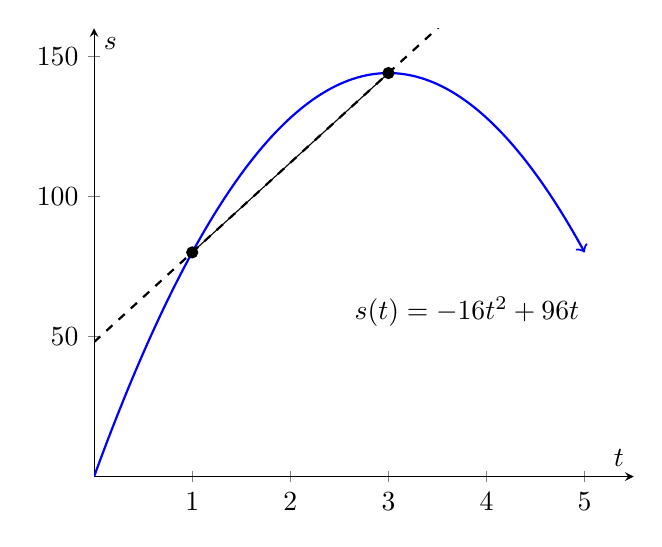
\begin{tikzpicture}
                \begin{axis}[
                	axis x line=middle,
                	xmax=5.5, xmin=0,
                	axis y line=center,
                	ymax=160, ymin=0,
                	xlabel=$t$,ylabel=$s$
                    ]
                    \addplot[name path=f,smooth,domain=0:5,color=blue,samples=100,->,thick] {-16*x^2 + 96*x};
                    \addplot[name path=f,smooth,domain=0:5,color=black,dashed,samples=100,thick] {32*x + 48}; 
		    \addplot[mark=*] coordinates {(1,80) (3,144)};
		    \draw (3.8,50) node[anchor=south] {$s(t)=-16t^2+96t$};
                \end{axis}
            \end{tikzpicture}
        \end{center}

We call such a line a \textbf{secant line}.

\vspace{5mm}

We can generalize the average velocity function to any function $f$. 

\vspace{5mm}

\boxenv{Average Rate of Change.}{Given a general function $f$ defined on $\ls a,b\rs$, the quantity

\vspace{15mm}
is called the \textbf{average rate of change} of $f$ on $\ls a,b \rs$.}

\vspace{5mm}

What if, instead of computing the average velocity between two time points, we want to compute the \textbf{instantaneous velocity} at a particular time? We cannot do this through standard means\dots

\vspace{10mm}

\Example Let's see if we can determine what the instantaneous velocity ``should be'' at a particular time. Suppose we want the instantaneous velocity at $t=1$ second after the rock was launched.
\\
\begin{center}
\renewcommand{\arraystretch}{1.5}
\begin{tabular}{|c|c|}
\hline
\rowcolor[HTML]{EFEFEF} 
$[1,t_1]$ & $\displaystyle\frac{s(t_1)-s(1)}{t_1-1}$  \\ \hline 
%$[1,2.000]$                     & 48.000 \pause                             \\  \hline 
$[1,1.500]$                & \phantom{56.000}                                \\  \hline 
$[1,1.100]$                   & \phantom{62.400}                                \\ \hline 
$[1,1.010]$                  & \phantom{63.840}                                \\  \hline 
$[1,1.001]$                 & \phantom{63.984}                                \\ \hline 
\end{tabular}
\end{center}

\newpage 

What is the pattern as $t_1$ approaches $1$, i.e.\ $t_1\to 1$?

\vspace{15mm}

\Example Suppose $f(x)=\disp\frac{2x-8}{\sqrt{x}-2}$. The following table was constructed for different values of $x$.

\begin{center}
\begin{tabular}{|
>{\columncolor[HTML]{EFEFEF}}c |c|c|c|c|c|c|c|}
\hline
$x$    & 3.7 & 3.8 & 3.9 & 4.0 & 4.1 & 4.2 & 4.3 \\ \hline
$f(x)$ & 7.847 & 7.899 & 7.950 & {\color{red}{$0/0$}} & 8.050 & 8.099 & 8.147 \\ \hline
\end{tabular}
\end{center}

How can we express the limit of $f(x)$ using limit notation?

\vspace{20mm}

As we progress through the course, we will see that every fundamental task in calculus involves the calculation of a \textbf{limit}!

\subsection*{Tangent Lines}

\boxenv{Definition.}{A \textbf{tangent line} to a curve at a point $P(x,y)$ is a line that ``just touches'' the curve at $P$ and has the same direction as the curve.}

\vspace{5mm}

Tangent lines can help us see the geometric connection between \textbf{average} and \textbf{instantaneous} velocity. As the time interval for an average velocity shrinks, the slope of the associated \textit{secant} line  approaches the slope of the \textit{tangent} line at the point of instantaneous velocity.

$$\color{blue} s(t)=-16t^2+96t$$
         \begin{center}
            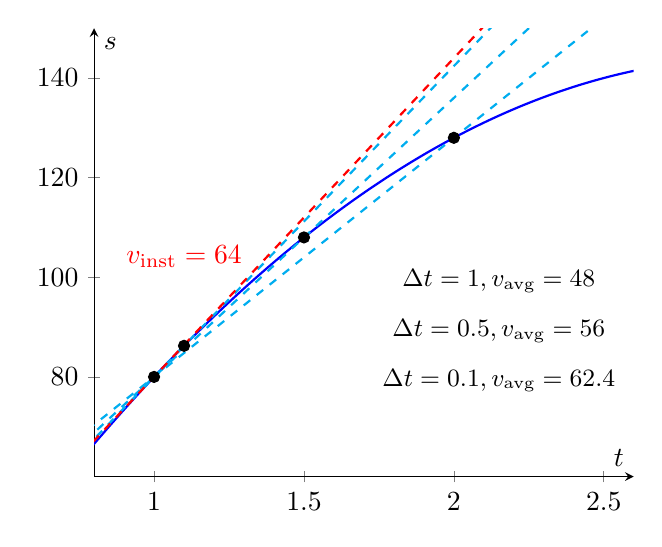
\begin{tikzpicture}[scale=1]
                \begin{axis}[
                	axis x line=middle,
                	xmax=2.6, xmin=0.8,
                	axis y line=center,
                	ymax=150, ymin=60,
                	xlabel=$t$,ylabel=$s$
                    ]
                    \addplot[name path=f,smooth,domain=0:5,color=blue,samples=100,->,thick] {-16*x^2 + 96*x};
                    \addplot[name path=f,smooth,domain=0:5,color=cyan,dashed,samples=100,thick] {48*(x-1) + 80};
                    \addplot[name path=f,smooth,domain=0:5,color=cyan,dashed,samples=100,thick] {56*(x-1) + 80};
                    \addplot[name path=f,smooth,domain=0:5,color=cyan,dashed,samples=100,thick] {62.4*(x-1) + 80};
                \addplot[name path=f,smooth,domain=0:5,color=red,dashed,samples=100,thick] {64*(x-1) + 80};

		    \addplot[mark=*] coordinates {(1,80)};
		    \addplot[mark=*] coordinates {(1.1,86.24)};
		    \addplot[mark=*] coordinates {(1.5,108)};
		    \addplot[mark=*] coordinates {(2,128)};
		    \draw[color=red] (1.1,100) node[anchor=south] {$v_{\text{inst}}=64$};
		    
		    \draw (2.15,95) node[anchor=south] {\small $\Delta t = 1, v_{\text{avg}} = 48$};
		    \draw (2.15,85) node[anchor=south] {\small $\Delta t = 0.5, v_{\text{avg}} = 56$};
		    \draw (2.15,75) node[anchor=south] {\small $\Delta t = 0.1, v_{\text{avg}} = 62.4$};
                \end{axis}
            \end{tikzpicture}
            
            \vspace{3mm}
            
View an interactive demo here: \url{https://www.desmos.com/calculator/gfpvpjeksy}
        \end{center}
        
        
\newpage

\textbf{Summary}
\begin{itemize}
	\item Informally, a \textbf{limit} is the ``expected output'' of a function or expression that cannot be directly calculated. We write this limit as 
	$$\lim_{x\to c} f(x)=L.$$
	
	\item The \textbf{instantaneous velocity} is the limit of the average velocity as the time interval shrinks to zero.
	$$v_{\text{inst}}=\lim_{t_2\to t_1}\frac{s(t_2)-s(t_1)}{t_2-t_1}$$
	
	\item Geometrically, for two points $P$ and $Q$\dots
	\begin{itemize}
		\item the \textbf{average} velocity is the slope of the \textbf{secant} line passing through $PQ$, and
		\item the \textbf{instantaneous} velocity is the slope of the \textbf{tangent} line passing through $P$.
	\end{itemize}
	\item Calculating the slope of a tangent line is not possible through standard algebraic means. Our study of \textbf{calculus} with introduce techniques for finding the slope of a tangent line.

\end{itemize}

\vspace{5mm}

\textbf{Helpful Equations.} The following equations from an algebra course will be useful when working with secant and tangent lines.
\begin{itemize}
\item \textbf{Slope of a Line.}
$$m=\frac{\Delta y}{\Delta x}=\frac{y_2-y_1}{x_2-x_1}=\frac{y_1-y_2}{x_1-x_2}$$
\item \textbf{Slope Intercept Form.}
$$y=mx+b$$
\item \textbf{Point-Slope Form.}
$$y-y_1=m(x-x_1)$$
\end{itemize}
\end{document}